\documentclass{article}

\title{TikZ 矢量子系统}
\author{soma-typeset}
\date{2026-11-25}

\begin{document}

\section{一张与 PGF 对齐的图}

下面这段 \verb|tikzpicture| 与 \verb|examples/tikz/figure.tex| 逐字相同，
后者由 \verb|pdflatex| 排出参考图。坐标、线宽、虚线、填充、圆、节点锚点与
箭头都由整数几何计算，不经过浮点，也不依赖外部图片。

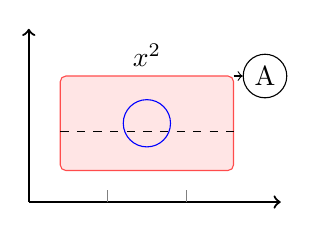
\begin{tikzpicture}
  % axes
  \draw[->, thick] (0,0) -- (3.2,0);
  \draw[->, thick] (0,0) -- (0,2.2);
  % panel with a rounded, filled rectangle
  \draw[red!70, fill=red!10, rounded corners=2pt]
    (0.4,0.4) rectangle (2.6,1.6);
  % dashed baseline inside the panel
  \draw[dashed] (0.4,0.9) -- (2.6,0.9);
  % circle and node
  \draw[blue] (1.5,1.0) circle (0.3);
  \node[draw, circle, inner sep=2pt] (A) at (3.0,1.6) {A};
  \draw[->] (2.6,1.6) -- (A.west);
  % tick marks
  \foreach \x in {1,2} {\draw[gray] (\x,0) -- (\x,0.15);}
  % label
  \node[above] at (1.5,1.6) {$x^2$};
\end{tikzpicture}

节点文字走数学子系统：\verb|$x^2$| 是真正的公式，普通文字按正文字号排。
节点是图的原子单位，只随显示对象整体分页，不会从中断开。

\section{网格}

\verb|grid| 在起点与对角之间按步长画格线，默认 1\,cm，边界线总会画出：

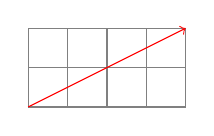
\begin{tikzpicture}
  \draw[step=0.5, gray] (0,0) grid (2,1);
  \draw[red, ->] (0,0) -- (2,1);
\end{tikzpicture}

步长为零或格线超过一万条是硬错误；不认识的键同样是硬错误，图会退回为可见的
源码文本，而不是画错。

\end{document}
